\documentclass{article}
\usepackage[utf8]{inputenc}
\usepackage[T1]{fontenc}

\usepackage{fullpage}

\usepackage{tikz}
%\usetikzlibrary{calc,arrows,shapes,backgrounds,patterns,fit,decorations,decorations.pathmorphing}

\usepackage[shadow,colorinlistoftodos,textwidth=2.5cm]{todonotes}
\usepackage[final,colorlinks,hyperindex,unicode=true,pdftitle=SPAdes Manual]{hyperref}
\usepackage{url}
\usepackage{booktabs}

\usepackage{cleveref}

\def\spades{SPAdes}
\def\bh{BayesHammer}
\def\ecoli{\it E.~coli}

\usepackage{textcomp}
\usepackage{listings}
\definecolor{light-gray}{gray}{0.92}
\lstset{
  upquote=true,
  columns=fullflexible,
  basicstyle=\ttfamily,
  framerule=0pt,
  frame=single,
  backgroundcolor=\color{light-gray},
  literate={*}{{\char42}}1
           {-}{{\char45}}1
}

%\usepackage[space=true]{accsupp}
%% requires the latest version of package accsupp
%\newcommand{\copyablespace}{
%    \BeginAccSupp{method=hex,unicode,ActualText=00A0}
%\ %
%    \EndAccSupp{}
%}


%\newenvironment{mycode}
%  {\begin{lstlisting}}
%  {\end{lstlisting}}

\begin{document}
\sloppy

\title{{\spades} 2.0.1 Manual\\{\small 
  Revision: \today}}
\date{}
\author{}
\maketitle

{\spades} stands for St.~Petersburg genome assembler.
It is intended for both single cell MDA and standard (multicell) 
assemblies. 
%{\spades} comes with error correction tool called BayesHammer. 
This manual will help you to install and run
{\spades}. The latest version of the manual can be downloaded at \url{http://bioinf.spbau.ru/spades}.


\renewcommand{\contentsname}{}
\tableofcontents

%\pagebreak

%\listoftodos

\pagebreak

\section{General setting}
\subsection{Notation}
{\spades} works with single and forward-reverse paired end reads.
The following picture explains the notions of 
read length, distance, gap, and insert size
for forward-reverse paired end reads.

\begin{center}
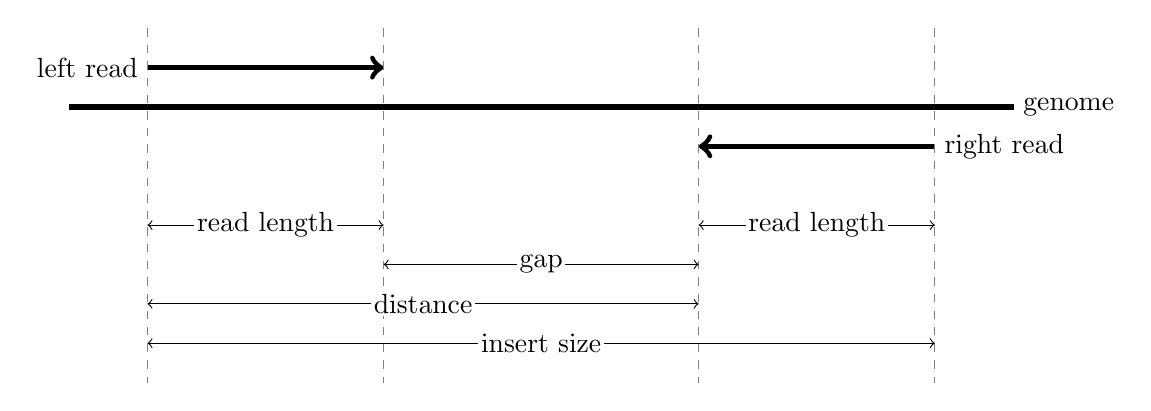
\begin{tikzpicture}
%\draw[help lines] (0,-3) grid (10,3);
\draw[line width=2pt] (-1,2) -- (11,2);
\draw[line width=2pt,->] (0,2.5) -- (3,2.5);
\draw[line width=2pt,->] (10,1.5) -- (7,1.5);

\node[rectangle,anchor=east] at (0,2.5) {left read};
\node[rectangle,anchor=west] at (11,2) {genome};
\node[rectangle,anchor=west] at (10,1.5) {right read};

\foreach \x in {0, 3, 7, 10}
  \draw[dashed,gray] (\x,3) -- (\x,-1.5);

\foreach \f/\s/\y/\t in {0/3/0.5/read length, 7/10/0.5/read length, 3/7/0/gap, 0/7/-0.5/distance, 0/10/-1/insert size}
\path[<->,draw] (\f,\y) -- node[fill=white,inner sep=1pt,rectangle] {\t} (\s,\y);
\end{tikzpicture}
\end{center}

\subsection{Config files and commands}
Config files and commands are given in gray boxes. 
In config files, the part of a line starting with a semicolon is a comment.

Note: text can be copy-pasted directly from this document
and all URLs and links to sections in the manual are clickable.


\section{Requirements}
\subsection{Operating system}
{\spades} requires a 64-bit Linux system.
%You need to have root privileges in order to install {\spades}.

\subsection{RAM}
Assembling our test multi-cell {\ecoli} dataset 
by {\spades} uses about 700~Mb peak memory, and single cell
{\ecoli} dataset uses 6~Gb peak memory. 
Correcting errors in these datasets requires about 70~Gb of RAM.
These datasets can be found at \url{http://spades.bioinf.spbau.ru/spades_test_datasets}.

\section{Installing {\spades}}
Each of the following subsections describes a way of installing {\spades}.
If you have root priveleges then proceed to either \cref{subsec:deb_package}
or \cref{subsec:rpm_package} to install a Debian or RPM package.
\Cref{subsec:archive} provides a way to build {\spades}
from the source code. This does not require rot priveleges, but 
you will have to install also some libraries that {\spades} depends on.
Finally, in \cref{subsec:binaries} it is described how one can just 
download the binaries.


\subsection{Installing Debian package (for Debian, Mint, Ubuntu, etc)}\label{subsec:deb_package}
First, add the repository containing {\spades} by inserting the following line
to the end of the file {\tt /etc/apt/sources.list}
\begin{lstlisting}
deb http://debian.bioinf.spbau.ru /
\end{lstlisting}
Note that the space before the last slash is required. 
Update the package list by typing
\begin{lstlisting}
sudo apt-get update
\end{lstlisting}
After that, {\spades} can be installed just by typing
\begin{lstlisting}
sudo apt-get install spades
\end{lstlisting}

\subsection{Installing RPM package (for CentOS, Fedora, Mandriva, Red Hat, SUSE, etc)}\label{subsec:rpm_package}
If your Linux system can install RPM packages you can use {\tt spades.rpm}
at \url{http://spades.bioinf.spbau.ru/release2.0.1/spades.rpm}. Use a front-end
such as {\tt yum}, {\tt Zypper}, or {\tt apt-rpm} to install this package.
The list of available front ends to RPM are given at, e.g.,
\url{http://en.wikipedia.org/wiki/RPM_Package_Manager#Front_ends}.

\subsection{Running {\spades} without installation (building from source)}\label{subsec:archive}
If you're unable to install a package (e.g., you don't have root privileges),
you can download {\spades} as an archive (\url{http://spades.bioinf.spbau.ru/release2.0.1/spades_2.0.1.tar.gz}) and just extract it.
Downloading and extracting from the command line is done as follows:
\begin{lstlisting}
wget http://spades.bioinf.spbau.ru/release2.0.1/spades_2.0.1.tar.gz
tar -xzf http://spades.bioinf.spbau.ru/release2.0.1/spades_2.0.1.tar.gz
cd spades_2.0.1
\end{lstlisting}
In this case, you will have to take care of some dependencies beforehand:
\begin{itemize}
\item {\tt g++} (version 4.4 or higher)
\item {\tt python} (version 2.4 or higher)
\item {\tt cmake} (version 2.6 or higher)
\item {\tt boost} (version 1.42 or higher)
\item {\tt zlib}
\end{itemize}

\subsection{Running {\spades} without installation (even without building)}\label{subsec:binaries}

If you don't have possibility to install some of the packages described above,
we've prepared the {\spades} binaries for multiple values of $k$ (see 
\cref{subsec:assembly}),
in the range from 11 to 149. For our test datasets, we recommend $k = 21, 33, 55$.
To use these binaries, you need to download {\spades} as an archive (\url{http://spades.bioinf.spbau.ru/release2.0.1/spades_2.0.1.tar.gz}),
extract it and use the following scripts to download the binaries:
\begin{lstlisting}
./spades_download_binary.py <space-separated values of k>
./spades_download_bayeshammer.py
\end{lstlisting}

\section{Testing your installation}
For testing purposes, {\spades} comes with a toy dataset (first $1{,}000$ bp of {\ecoli}).
If you intalled {\spades} from package 
(see \cref{subsec:deb_package,subsec:rpm_package}) type
\begin{lstlisting}
spades.py
\end{lstlisting}
Otherwise, {\tt cd} to the folder where you extracted the archive to
(see \cref{subsec:archive,subsec:binaries}) and type
\begin{lstlisting}
./spades.py
\end{lstlisting}
It runs {\spades} on this toy dataset.
If the installation is successful you will see lines like the following lines in the end of the log.
\begin{lstlisting}

 * Corrected reads are in .../spades_output/ECOLI_1K/corrected/
 * Assembled contigs are .../spades_output/ECOLI_1K/spades_04.18_17.59.30/ECOLI_1K.fasta
 * Assessment of their quality is in 
.../spades_output/ECOLI_1K/spades_04.18_17.59.30/quality_results/quality.txt

Thank you for using SPAdes!

======= SPAdes pipeline finished
\end{lstlisting}



\section{Running {\spades}}\label{sec:running}
To run {\spades} type
\begin{lstlisting}
spades.py <config.info>
\end{lstlisting}
if you intalled {\spades} from package (see \cref{subsec:deb_package,subsec:rpm_package}), or 
\begin{lstlisting}
./spades.py <config.info>
\end{lstlisting}
from folder you extracted the archive (see \cref{subsec:archive,subsec:binaries}).
By default (i.e., if no config file is given) {\spades} uses the file {\tt spades\_config.info}. 
If {\spades} was installed from package the default config file is located at {\tt  /usr/share/spades/spades\_config.info}, otherwise it can be found in the folder 
where {\spades} was extracted to.


Below we first give an example of a config file
and then explain its contents in detail. The parameters that
are necessary to adjust to run {\spades} on your dataset are given in blue.

\lstset{emph={paired_reads,single_reads,single_cell,reference,genes,operons}, emphstyle=\color{blue}}

\begin{lstlisting}													
; all paths are relative to the working directory but you can also use $cfg variable 
; to set paths relative to this config

project_name        ECOLI_1K                          ; optional. Name of this config file is used if not specified
output_dir          ./spades_output

dataset
{
    paired_reads        $cfg/test_dataset/ecoli_1K_1.fq.gz $cfg/test_dataset/ecoli_1K_2.fq.gz
    single_reads                                      ; optional
    single_cell         false
}

assembly
{
    iterative_K         21 33 55
    paired_mode         true
    generate_sam_files  true                          ; optional. Default is false
    gap_closer          true                          ; optional. Default is true
}

; optional. If this section exists (even if it is empty), spades.py 
; evaluates quality of the final contigs
quality_assessment      
{
    reference           $cfg/test_dataset/reference_1K.fa.gz     ; optional
    genes               $cfg/test_dataset/genes_1K.txt           ; optional
    operons             $cfg/test_dataset/operons_1K.txt         ; optional
}
\end{lstlisting}

The four sections of the config file contain dataset settings
and setting of three stages of {\spades} pipeline~--- error correction,
assembly, and quality estimation.
To run only some of these three stages just remove (or comment or rename) unnecessary stages.
If you run {\spades} with the same {\tt output\_dir} and {\tt project\_name} as one of previous runs, it checks if you have already made the error correction stage and asks if you want to correct the reads again.

The two global variables are the following
\begin{description}
\item[{\tt project\_name}] specifies the name of the project. It is recommended to set a meaningful name for each separate project.
It makes it easier to find the results in the output folder.
\item[{\tt output\_dir}] specifies the output folder.
\end{description}

\subsection{Dataset settings}
{\spades} accepts single reads as well as forward-reverse paired end reads
in FASTA and FASTQ format; however, in order to run error correction, reads should be in FASTQ format. All files may be compressed with gzip.
At present, {\spades} can accept only one paired-end library as input.

\begin{lstlisting}													
dataset
{
    paired_reads        $cfg/test_dataset/ecoli_1K_1.fq.gz $cfg/test_dataset/ecoli_1K_2.fq.gz
    single_reads                                      ; optional
    single_cell         false
}
\end{lstlisting}

\begin{description}
\item[{\tt paired\_reads}] specifies input paired end reads organized into one or two files.
\begin{itemize}
\item If using a single file, interlace the corresponding mated ``1'' and ``2'' reads. Put the read from the Illumina file {\tt s\_n\_1\_export.txt} first, followed by the read from the Illumina file {\tt s\_n\_2\_export.txt}.
\item If using a pair of files, the first file should have the Illumina ``1'' subreads and the second file should have the Illumina ``2'' subreads, with corresponding reads in the exact same order.  The two filenames should be separated by a space.
\end{itemize}
\item[{\tt single\_reads}] specifies reads without pairs. You can specify any number of
files with single reads. File names should be separated by spaces.
\item[{\tt single\_cell}] flag is set if input data was obtained with MDA (single cell) technology.
\end{description}

\subsection{Error correction settings}
The section {\tt error\_correction}) is responsible for correcting errors in the input reads;
error correction in the {\spades} pipeline is done with {\bh}, a recently developed error correction tool that works well for the case of non-uniform coverage
(e.g., on single-cell data); you can find more information about {\bh} at \url{http://bioinf.spbau.ru/en/spades/bayeshammer}.
Note that for an accurate assembly it is important to use this stage, especially for single-cell datasets.

\begin{lstlisting}
error_correction
{
    tmp_dir                                           ; optional. <output_dir>/corrected/tmp is used if not specified
    qvoffset                                          ; optional. Either 33 or 64
    max_iterations      2
    max_threads         16
    max_memory          250                           ; in GB
    gzip_output         true ; optional
}
\end{lstlisting}

\begin{description}
\item[{\tt tmp\_dir}] specifies the directory where temporary files are stored. Note that {\bh} uses a significant amount of disk space (even though it
cleans up after itself) so you might want to consider setting {\tt tmp\_dir} to something other than {\tt /tmp} (e.~g. external drive).
\item[{\tt qvoffset}] sets PHRED quality offset in the input reads ($33$ or $64$). If not given, {\bh} tries to find this value automatically.
\item[{\tt max\_iterations}] sets the maximum number of iterations
for the error correction procedure. Usually, the second iteration does improve upon the first, but then there is almost no change.
\item[{\tt max\_threads}] sets the maximum number of threads.
\item[{\tt max\_memory}] sets the maximum amount of available RAM (in Gb). {\bh} (and the entire {\spades} pipeline) will fail if it attempts
to allocate more RAM than specified here.
\item[{\tt gzip\_output}] flag forces {\bh} to output compressed corrected reads (with {\tt gzip}).
\end{description}

\subsection{Assembly settings}\label{subsec:assembly}
The section {\tt assembly} allows to change the assembly settings. 

\begin{lstlisting}
assembly
{
    iterative_K         21 33 55
    paired_mode         true
    generate_sam_files  true                          ; optional. Default is false
    gap_closer          true                          ; optional. Default is true
}
\end{lstlisting}

\begin{description}
\item[{\tt iterative\_K}] specifies one or more odd values for $k$-mer (vertex) sizes.  Informally, smaller values of $k$ make the graph more connected,
but at the same time more tangled, while higher values of $k$ may defragment the graph, but allow to resolve short repeats.
The typical value for this variable is {\tt 21 33 55}. See the paper~\cite{main} for more details.
Note that in the configuration file, $k$ is the size of a vertex, while in the paper, $k$ is the size of an edge (i.e., larger by one).

\item[{\tt paired\_mode}] turns the repeat resolver on/off if parameter set to true/false.

\item[{\tt generate\_sam\_files}] flag forces {\spades} to generate a SAM-file
showing how the paired reads specified in dataset section of config file are aligned to resulting contigs.  Alignments from this SAM-file
can be visualized, e.g., by Tablet~\cite{tablet}.

\item[{\tt gap\_closer}] turns the gap closer on/off. This module restores $k$-mers that are not covered not by whole reads
but by overlapping parts of two reads and are supported by paired reads. This is efficient when a library has a small insert size (up to 3x read length). If insert size is large, you can turn 
it off to slightly decrease the runing time of {\spades}.
Note: you can decrease the running time of {\spades} by setting just one value of $k$ (say, 55) and turning the gap closer on
(since the gap closer usually gives similar results as running with several smaller values of $k$).
\end{description}

\subsection{Quality assessment settings}\label{subsection:qualitysetting}
The section {\tt quality\_assessment}
is needed to estimate the quality of the resulting assembly.

\begin{lstlisting}
; optional. If this section exists (even if it is empty), spades.py 
; evaluates quality of the final contigs
quality_assessment      
{
    reference           $cfg/test_dataset/reference_1K.fa.gz     ; optional
    genes               $cfg/test_dataset/genes_1K.txt           ; optional
    operons             $cfg/test_dataset/operons_1K.txt         ; optional
}
\end{lstlisting}


If this section is present in the config file then
{\spades} evaluates assembly results by computing various metrics (e.g., N50, NG50, number of long ORFs, etc.) on the resulting contigs.
The variables {\tt reference}, {\tt genes}, and {\tt operons} are self-explanatory.

{\tt genes} and {\tt operons} should be either in GFF format (versions 2 
(\url{http://www.sanger.ac.uk/resources/software/gff/spec.html} and 3 (\url{http://www.sequenceontology.org/gff3.shtml}) are supported) or in plain TXT format 
with 4 tab-separated columns: {\bf the chromosome name} (it should match the exact string in the reference file), {\bf gene or operon id}, {\bf start position} and
{\bf end postion} (the coordinates are 1-based and if {\bf start postion} < {\bf end postion} than that gene or operon is on the positive strand and it is on the negative strand otherwise).

Note that the quality is estimated even if this section is empty. Our quality tool uses Plantagora (\url{http://www.plantagora.org/}) and MUMmer (\url{http://mummer.sourceforge.net/}).

The computed metrics are described in detail in \cref{section:metrics}.

\subsection{Creating a config file for your dataset}
To create a config file for your dataset {\tt cd} to the {\spades} folder
and copy the default config file to a new file:
\begin{lstlisting}
cp spades_config.info your_project_name.info
\end{lstlisting}
Then edit this new file and set all the parameters
shown in blue in \cref{sec:running}.

%You can then run {\spades} by typing
%\begin{lstlisting}
%spades.py your_project_name.info
%\end{lstlisting}

\section{Assembly quality metrics}\label{section:metrics}
In this section, we describe various metrics computed by the quality tool
of {\spades} pipeline (see \cref{subsection:qualitysetting}). Note that 
the metrics based on the reference are computed only if the reference is given
in the config file.

\begin{description}
\item[N50] is the contig length such that using longer or equal length contigs
produces half (50\%) the bases of the assembly.  Usually there is no
value that produces exactly 50\%, so the more technical definition is
the minimal length $x$ such that using contigs of length at least $x$ accounts for at least 50\% of the total assembly length.

\item[NG50] is the contig length such that using longer or equal length contigs
produces half (50\%) the bases of the reference genome.

\item[N75 and NG75] are defined similarly with 75\% instead of 50\%.

\item[Number of contigs] is the total number of contigs in the assembly.

\item[Largest contig] is the length of the longest contig in the assembly.

\item[Total length] is the total number of bases in the assembly.

\item[Reference length] is the total number of bases in the reference.

\item[Average \%IDY] is the average of alignment identity percent (quality) among all contigs.

\item[Misassemblies] gives the number of positions at the assembled contigs where the left
flanking sequence aligns over 1kb away from the right flanking sequence on the
reference or they overlap on more than 1 kb or flanking sequences align on different strands.

\item[Misassembled contigs] is the number of contigs that contain misassembly
events.

\item[Misassembled contig bases] is the number of total bases contained in all
contigs that have one or more misassemblies.

\item[Unaligned contigs] is the number of contigs that have no alignment to the
reference sequence.  The value ``$X$ ($Y$ partial) ($Z$)'' means:
$X$ totally unaligned contigs
plus $Y$ partially unaligned contigs
and the total number of unaligned bases is $Z$.

\item[Ambiguous contigs] is the number of contigs that have reference alignments
of equal quality in multiple locations on the reference.
The value "$X$ ($Y$)" means $X$ ambiguous contigs with $Y$ bases in them.

\item[NA50] (A stands for ``aligned'') is 
defined similarly to N50 but only
lengths of aligned blocks are counted.
If a contig has a misassembly with respect to the reference, it is broken into smaller pieces.
If a contig has bases that do not align to the reference, they are not counted
in NA*, NGA*. NGA50, NA75, NGA75 are defined in the same way.

\item[Mapped genome (\%)] is the ratio of the total number of aligned bp in the assembly
to the genome size.  Short contigs (less than 500~bp) that map to multiple
places may be counted many times in this quantity.  A base in the genome is
counted as aligned one if there is at least one contig with at least one
alignment with this base.

\item[Genes] is the number of genes in the assembly (full and partial), based
on the positions the contigs map to in the reference genome with an annotated
list of genes. The value ``$X$ + $Y$ partial'' means $X$ full genes and $Y$ partial ones
(at least 100 bases are aligned).

\item[Operons] is the number of operons in the assembly (full and partial),
based on the positions the contigs map to in the reference genome with an annotated list of operons.
The value ``$X$ + $Y$ partial'' means $X$ full operons and $Y$ partial ones (at least 100 bases are aligned).

\item[Number of miscalled] is the number of miscalled bases (e.g. having ``C'' in the assembly and ``G'' in the genome).

\item[Number of uncalled] is the number of uncalled bases (``N'').

\item[Bases missed] is the number of missed bases (which are presented in the genome and missed in the assembly).

\end{description}

\section{Output}
Results can be found in the folder specified by {\tt output\_dir}.
Specific directories containing corrected reads, assembly, and quality estimate are shown at the end of the log. In the example with the toy dataset discussed above this is 
{\tt /usr/share/spades/spades\_output/ECOLI\_1K/}.


\section{Postprocessing}

\subsection{Correcting errors in the resulting contigs}
While {\spades} produces accurate assemblies, 
we recommend running SEQuel~\cite{sequel} after {\spades} to further reduce the number of small errors
(single nucleotide substitutions and small indels). SEQuel is available at
\url{http://bix.ucsd.edu/SEQuel/}. Note that one can set the flag {\tt generate\_sam} to {\spades}
(see \cref{subsec:assembly}) to generate a SAM-file showing how the 
reads are aligned to the resulting contigs. This file can then be given to SEQuel as input.

\subsection{Scaffolding}
The current version of {\spades} does not have a scaffolding stage.
One can use a separate scaffolder such as Opera~\cite{opera}.
It is available at \url{http://sourceforge.net/projects/operasf/}.

\section{Feedback and bug reports}
We will be thankful if you help us make {\spades} better
by sending your comments, bug reports, and suggestions to
\url{spades.support@bioinf.spbau.ru}.


\bibliographystyle{plain}
\bibliography{manualbib}


\end{document}
